\subsection{Round-Robin sin migración (RR2)}

RR sin migración es una variante del RR que no permite la migración de procesos
entre los núcleos.\\

En este algoritmo cuando un proceso nuevo empieza a correr le es asignado
un núcleo, el que esté 'más libre', es decir, tenga menos procesos asignados
(contando procesos en espera, corriendo y bloqueados).
Luego, durante toda su ejecución el proceso está ligado a ese núcleo.\\

Esta variante, como todo algoritmo de schedulling, tiene sus pros y sus contras.\\
Para simplificar las explicaciones y los gráficos tomamos ejemplos de 
dos núcleos, aunque esto puede ser expandido a más de dos.\\

\textbf{Contra - caso: Sobrecarga de un núcleo}\\
Una contra es que uno de los núcleos puede quedar 'sobrecargado' mientras el
otro no tiene ningún proceso asignado (está corriendo IDLE).

El lote de tareas utilizado tiene dos posibles procesos, uno que utiliza CPU durante muchos ciclos (proceso largo)
y otro que utiliza CPU durante unos pocos ciclos (proceso corto). Son en total 6 procesos, por simplicidad.\\
Si los procesos llegan alternandose entre largos y cortos entonces:
\begin{itemize}
\item Al primer proceso (largo) le es asignado el núcleo 0.
\item Al segundo proceso (corto) se le asigna el núcleo 1.
\item Al tercer proceso (largo) le es asignado el núcleo 0.

... y continúa así.
\end{itemize}

Con lo cuál, luego de la carga del último proceso quedan distribuidos de la siguiente manera:\\ 
Núcleo 0: 3 procesos largos. Núcleo 1: 3 procesos cortos.

En el ciclo 25 los procesos cortos son finalizados quedando el núcleo 0 con tres procesos y el 1 IDLE.\\

\textbf{RR2 (sin migración)}
\begin{center}
 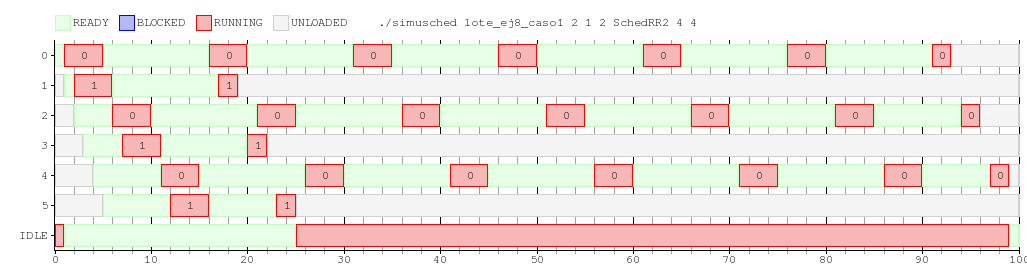
\includegraphics[scale=0.48]{./RR2/caso1RR2.png}
\end{center}

\textbf{RR (con migración)}
\begin{center}
 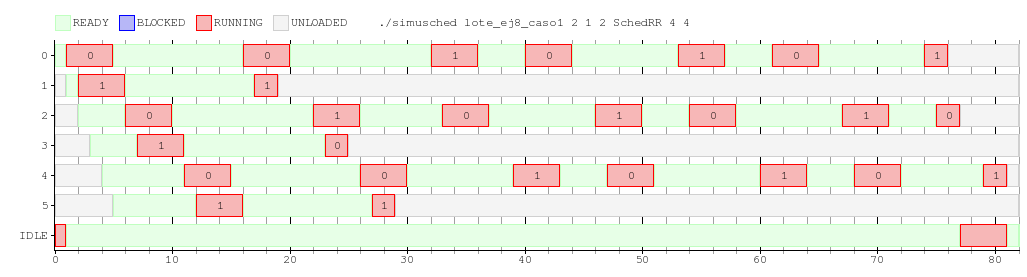
\includegraphics[scale=0.48]{./RR2/caso1RR.png}
\end{center}

Este escenario también se podría dar si en vez de tareas cortas tenemos tareas que realizan llamadas bloqueantes.
Entonces en el núcleo 0 hay tareas usando CPU y el núcleo 1 queda esperando que algún proceso se desbloquee.\\

\textbf{Pro - caso: Migración costosa}\\
Una de las ventajas de RR2 queda expuesta si el costo de la migración es grande.
Si los procesos cambian mucho entre núcleos puede que en el caso de RR 
el procesador pase más tiempo haciendo tareas de mantenimiento que efectivamente corriendo procesos.\\

Vamos a correr el experimento sobre el mismo lote de tareas y con los mismos
quantums que en el caso anterior, para que sea más obvio el cambio. Lo único
que vamos a variar es el costo de migración que va a pasar de 2 a 5.\\

\textbf{RR2 (sin migración)}
\begin{center}
 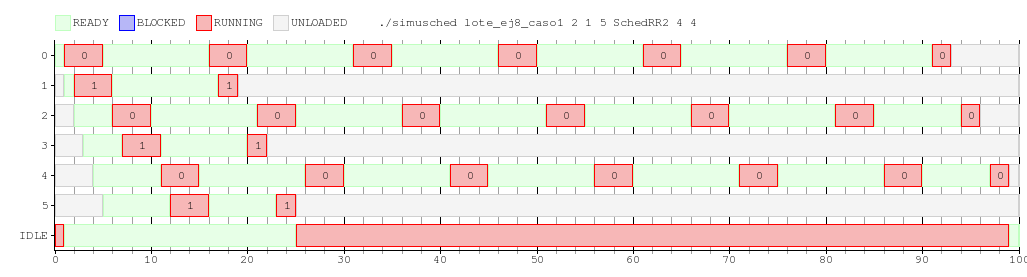
\includegraphics[scale=0.48]{./RR2/caso2RR2.png}
\end{center}

\textbf{RR (con migración)}
\begin{center}
 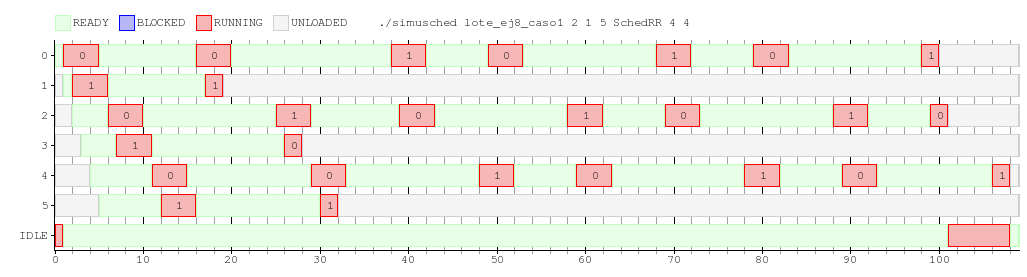
\includegraphics[scale=0.48]{./RR2/caso2RR.png}
\end{center}

No sólo RR2 termina apróx 10 ciclos antes; incluso bajo este lote de tareas que 
es un caso negativo; sino que además RR pasa mucho tiempo haciendo 
tareas de mantenimiento.